% Diese Zeile bitte -nicht- aendern.
\documentclass[course=asp]{aspdoc}

\graphicspath{{./Bilder/}}

%%%%%%%%%%%%%%%%%%%%%%%%%%%%%%%%%
%% TODO: Ersetzen Sie in den folgenden Zeilen die entsprechenden -Texte-
%% mit den richtigen Werten.
\newcommand{\theGroup}{Team 103 } % Beispiel: 42
\newcommand{\theNumber}{504: RSA} % Beispiel: A123
\author{Guo Linfeng \and Özakay Baris \and Julian Julian}
\date{Wintersemester 2022/23} % Beispiel: Wintersemester 2019/20
%%%%%%%%%%%%%%%%%%%%%%%%%%%%%%%%%

% Diese Zeile bitte -nicht- aendern.
\title{Gruppe \theGroup{} -- Abgabe zu Aufgabe \theNumber}

\begin{document}
\maketitle

\section{Einleitung}
Das Praktikum Aspekte der systemnahen Programmierung bei der Spieleentwicklung beschäftigt sich mit dem Programmieren von Prozessen auf niedriger Ebene. Dabei ist es wichtig die Schnittstellen zwischen Hardware and Software effektiv zu nutzen. Außerdem haben wir uns den Umgang mit der Assembly Programmiersprache AArch64 angeeignet und damit verbunden diverse Optimierungsmöglichkeiten für diese. Assembler ermöglicht die Assemblysprache in Maschinensprache zu übersetzten.Der Vorteil an einer derart Hardware-Nahen Programmierung ist, dass man eine viel bessere Leistung für seine Programme erzielen kann, da man angepasste Optimierungen treffen kann, zu welchen ein normaler Compiler aus einer Hochsprache nicht fähig ist. Diese Verbesserung spielt in vielen Bereichen der Informatik eine wichtige Rolle.

Das Praktikum bietet eine Vielzahl an Themengebiete. Eines davon, welchem wir uns gewidmet haben, ist die sogenannte Kryptographie. Kryptographie ist ein essentieller Bestandteil unserer heutigen Kommunikation. Einer der Algorithmen, der unter dem Fachgebiet der Kryptographie zum Einsatz kommt ist der RSA-Algorithmus. Der RSA-Algorithmus wurde im Jahr 1977 zum ersten Mal veröffentlicht und ist nach seinen Erfindern Rivest, Shamir und Adleman benannt. Die Relevanz des Algorithmus hat in der heutigen Zeit nicht nachtgelassen. Er wird in verschiedenen Bereichen wie zum Beispiel bei Banken, Webservern oder E-Mails, für Sicherheit und Datenschutz angewendet. Das Verfahren wird sehr oft für die Verschlüsselung der Kommunikation mit mehreren Teilnehmern genutzt. Dabei kommen zwei Schlüssel zum Einsatz, ein öffentlicher und ein privater Schlüssel. 

Ein Beispiel dazu: Person A und Person B wollen mit Hilfe des RSA Verfahrens mit einander kommunizieren. Angenommen alle öffentlichen Schlüssel stehen im Internet. A will eine Nachricht an B verschicken und sucht im Internet den öffentlichen Schlüssel von B heraus. Die Nachricht von A wird anschließend verschlüsselt und an B verschickt. Die verschlüsselte Nachricht kann nur von B entschlüsselt werden, da nur er den geheimen Schlüssel kennt. 
 
Ein Schlüssel ist ein Tupel. Der öffentliche Schlüssel ist durch das Tupel (e, N) und der geheimen Schlüssel durch das Tupel (d, N) gegeben. Dabei ist e der Verschlüsselungsexponent und d der Entschlüsselungsexponent. Für die Wahl dieser Variablen gibt es mehrere mathematischen Voraussetzung. Dabei müssen p und q jeweils Primzahlen sein.
\begin{align}
 N = p \cdot q
\end{align}
\begin{align}
1 < e < \varphi (N)
\end{align}
Außerdem muss e Teilerfremd zu $\varphi $(N) sein. $\varphi $(N) sei die Eulersche $\varphi $-Funktion.
\begin{align}
d \cdot e \equiv 1 \mod \varphi (N)
\end{align}
Nachdem man die Schlüssel generiert hat, kann man die Nachricht m mit Hilfe von e und N verschlüsseln und c ist die verschlüsselte Nachricht. Für die Entschlüsselung wird d verwendet.
\begin{align}
c {=} m^e \mod N
\end{align} 
\begin{align}
m {=} c^d \mod N
\end{align} 
An Hand eines Beispiels sehen wir wie die Nachricht m = 10 verschlüsselt wird. Wir wählen für N = 1363, e = 3 und d = 859. $\varphi $(1363) = 1288 und e ist zudem Teilerfremd. Mit (4) ergibt sich die verschlüsselte Nachricht 1000 = 10$^{3}$ $\mod $ 1288. Mit unserem geheimen Schlüssel wollen wir anschließend entschlüsseln. 1000$^{859}$ $\mod $ 1288 = m. Mit manueller Kalkulation ist das Ergebnis wie erwartet 10.

Der RSA-Algorithmus besteht aus vier Schritten: Schlüsselgenerierung, Schlüsselverteilung, Verschlüsseln und Entschlüsseln. Unsere Aufgabe ist die Generierung der drei Variablen d, e, N zu implementieren. Wir werden mit der Generation von N anfangen, gehen anschließend darauf ein wie die Variable e gewählt wird und zum Schluss wie man mit Hilfe vom erweiterten Euklidischen Algorithmus aus e und $\varphi $ (N) unser d erzeugt.

\section{Lösungsansatz}  
\subsection*{2.1 Primzahl Generierung }
Für die Wahl von N werden zwei Primezahl verwendet, p und q.

\subsection*{2.2 Wahl für e }
Der allererste RSA- Algorithmus stammt aus dem Jahr 1977. Diese Variante wurde ursprünglich so implementiert, dass man ein zufälliges d wählt und daraus e generiert. Allerdings ist diese Methode nicht sicher und e würde zu groß sein. Je kleiner bei diesem Algorithmus der Verschlüsselungsexponent e ist, desto schneller ist die Verschlüsselung. Eine große Zahl ist für die Verschlüsselung dennoch performant genug und erfüllt dabei auch die Sicherheitsanforderungen. Für die Wahl von e muss auf ein paar Voraussetzungen geachtet werden. Der Verschlüsselungsexponent muss größer als eins, und kleiner als $\varphi $(N) sein(1). Außerdem muss e teilerfremd zu $\varphi $(N) sein.

Damit der RSA- Algorithmus bessere Performance leistet und effizienter ist, muss e eine kurze Bit- Länge und ein kleines Hamming Gewicht haben. Das Hamming Gewicht bei einem String von Bits ist die Anzahl von Einsen. Die Bit Länge gibt die Anzahl an Bits, wenn eine Zahl in Binärschreibweise umgewandelt wird. Um diese Länge einer ganzen Zahl zu bestimmen, wird die folgende Formel verwendet:
\begin{align}
	bitLength(n) = \lfloor \log_{2}(n) + 1 \rfloor = \lceil \log_{2}(n + 1)\rceil
\end{align}
Der Grund für eine Verbesserung der Implementierung bei einem Verschlüsselungsexponent e mit einer kurzen Bit- Länge und einem kleinen Hamming Gewicht liegt an folgenden Eigenschaften:
\begin{itemize}
 \item [1.] Weniger Multiplikation: Um eine Nachricht zu entschlüsseln, muss man die Nachricht e- Fach mit sich selbst multiplizieren. Daher ist es weniger Rechenaufwand, falls e klein ist und verkürzt somit auch die Berechnungszeit.(3)
 \item [2.] Weniger Modulo Reduktion: Nach der Berechnung von $m^{e}$ wird die Operation Modulo N ausgeführt. Wenn e eine kurze Bit Länge hat, so muss weniger Modulo Reduktionen durchgeführt werden. Eine Potenz Modulo Berechnung hat eine Zeitkomplexität von O(log y). Dabei sei y der Exponent.   
 \item [3.] Kleineres Hamming Gewicht: Ein kleineres Hamming Gewicht bedeutet, dass die Zahl in der Bit- Schreibweise mehr Null- Bits hat. Dies spart ebenfalls Rechenaufwand bei der Potenzrechnung und der Modulo Operation.
\end{itemize}
Die meisten gewählten Zahlen für e sind 65537 und 3. 65537 ist groß genug und kann für die Sicherheit der Verschlüsselung sorgen. Zudem hat diese Zahl ein kleines Hammning Gewicht, in Binärschreibweis 0b10000000000000001. Die kleinste Zahl für e ist die drei. Drei hat ein Hamming Gewicht von zwei, 0b11, und ist somit für die Verschlüsselung sehr schnell. Allerdings ist die Verwendung diese Zahl nicht sicher für das RSA- Verfahren. %%%%%%%%%warum wird drei verwendet 

Bei unsere Implementierung haben wir zunächst geschaut ob unsere $\varphi $(N) größer ist als 65537 oder ob 65537 kleiner gleich $\varphi $(N) ist. Falls es kleiner gleich ist, wird e = 3 gesetzt. Im anderen Fall ist e = 65537.
\subsection*{2.2.1 Camicael Funktion} 
Für die Berechnung von $\varphi $(N) wird die Eulersche $\varphi $- Funktion verwendet. Die $\varphi $ Funktion gibt die obere Schranke für e an. Es gibt neben der Eulersche $\varphi $- Funktion noch eine weitere Funktion, um die obere Schranke für e bestimmt, die Carmicael Funktion, auch $\lambda $- Funktion genannt. Diese Funktion berechnet den kleinsten positiven Quotienten der $\varphi $- Funktion aus und optimiert somit die obere Grenze. In der unteren Graphik kann man sehen, dass der Wert von $\lambda $(N) ist in den meisten Fällen kleiner ist als  $\varphi $(N). So kann e möglichst klein gewählt werden. Je kleiner e, desto schneller ist die Verschlüsselung. 
\begin{figure}[h]
\centering
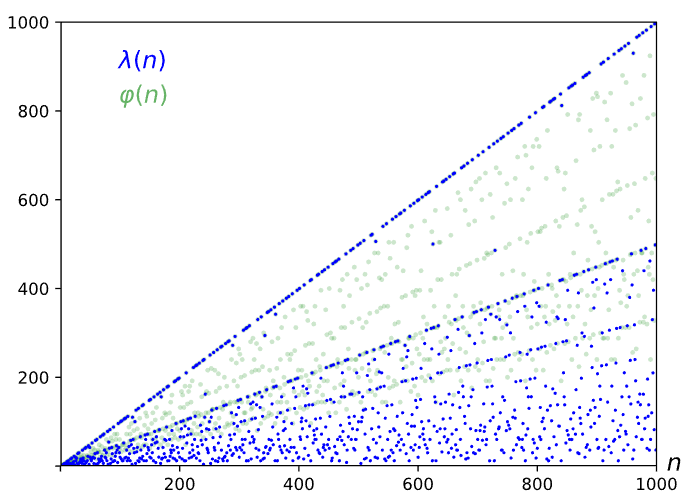
\includegraphics[scale = 0.6]{CarmichaelLambda.png}
\caption{Vergleich zwischen $\varphi $(N) und $\lambda $(N)}
\end{figure}

Die Formel für die Carmicael- Funktion sieht wie folgt aus:
\begin{align}
	g^m = 1 \mod n
\end{align} 
Dabei ist n der Eingabewert der Funktion. g sind alle teilerfremden Zahl zu n, welchen in der Funktion berechnet werden. m ist der Rückgabewert. Zur Implementierung der Carmicael Funktion haben wir zunächst die gcd()- Funktion als Hilfsmethode implementiert, welche den größten gemeinsamen Teiler zwischen zwei Zahlen a und b bestimmt. Falls das Ergebnis gleich eins ergibt, bedeutet dies, dass beide Zahlen teilerfremd sind und a kann so als g verwendet werden. Die Implementierung des Algorithmus ist einfach gehalten. Sie beinhaltet einen for- Loop, für die Überprüfung von allen teilerfremden Zahlen die kleiner als n sind und einen while- Loop, der Überprüft bei welchem Exponenten die Eigenschaft von (7) erfüllt wird. Falls eine teilerfremde Zahl gefunden wird, wird nach dem Bestimmen des Exponenten der Rückgabewert k aktualisiert. Dabei wird das kleinste gemeinsame Vielfache zwischen k und dem Exponenten berechnet. 

So war die eigentliche Implementierung. Jedoch sind wir bei dieser Art von Implementierung auf ein Problem gestoßen, denn es funktioniert nur für kleine Zahl, in eine Größenordnung von sechs. Deshalb haben wir letztendlich für eine andere Implementierungsvariante der $\lambda $ Funktion entschieden, mit der folgende Formel:
\begin{align}
	\lambda(N) = \frac{{p-1}\cdot{q-1}}{gcd(p-1, q-1)}
\end{align} 
Diese Implementierung nimmt die zwei Parameter p und q als Eingabe und berechnet mit Hilfe von der gcd- Funktion den $\lambda $ Wert. Die andere Implementierung dient ledigtlich nur als Hilfe und wird im richtigen Code nicht verwendet.
\subsection*{2.3 Der erweiterte Euklidische Algorithmus}
Bevor wir mit dem erweiterten Euklidischen Algorithmus beginnen, sollten wir zunächst verstehen, was der Euklidische Algorithmus bewirkt. Er ist der effizienteste Weg, um den größten gemeinsamen Teiler GCD zwischen zwei Zahlen zu bestimmen. In unserer Aufgabe müssen wir prüfen, ob die obere Schranke phi(N) und unser Verschlüsselungsexponent e teilerfremd sind. Die grundlegende Idee des Euklidischen Algorithmus ist, dass man den größten gemeinsamen Teiler zwischen zwei Zahlen bestimmt. Das Verfahren ist wie folgt:
\begin{itemize}
 \item [1.] Die Funktion bekommt zwei Eingaben, a und b. Daraus berechnet man sich r, welcher den Rest von der Division zwischen a und b bildet.
 \item [2.] Falls r gleich null ist, ist der größte gemeinsame Teiler von a und b gleich b und wir geben ihn als Ausgabe aus.
 \item [3.] Falls r nicht gleich null ist, ersetzen wir a durch b und b durch r und beginnen erneut bei Schritt 1. 
\end{itemize}
Wie der Name schon verrät, ist der erweiterte Euklidische Algorithmus eine Erweiterung des ursprünglichen Euklidischen Algorithmus. Beide Verfahren berechnen den GCD zwischen zwei ganzen Zahlen. Der erweiterte Algorithmus gibt uns außerdem noch den Koeffizienten der Bezout-Identität an. Es sind zwei ganze Zahlen x und y und stehen wie folgt im Zusammenhang:
\begin{align}
	ax + by = gcd(a, b)
\end{align} 
Wenn man die zwei Variable a und b hat, kann man x und y mit Hilfe von modulo multiplikative Inverse berechnen.

Die Implementierung vom EEA funktioniert wie folgt. Wir initialisieren zuerst x = 1 und y = 0. Diese sind unsere Koeffizienten der Bezout-Identität. Wir führen den euklidischen Algorithmus aus. Bei jedem Schritt werden außerdem die zwei Koeffizienten x und y mit folgender Formel aktualisiert. 
\begin{align}
	x_{new} = y, y_{new} = x - (floor(r/s)) \cdot y
\end{align} 
Die Variablen r und s sind Reste und Divisor des euklidischen Algorithmus. Die Funktion floor() gibt die größte Zahl, die kleiner als der Eingabewert ist, zurück. 
Wenn der euklidische Algorithmus terminiert, erhälten man das Ergebnis von GCD und die zwei Koeffizienten der Bezout-Identität, x und y. Für die Modulo Inverse von a $\mod$ b kann man mit Hilfe von x $\mod$ b berechnen, falls gcd(a,b) = 1 ist. Im anderen Fall gibt es keine Modulo Inverse.
 
In unsere Aufgabe sieht die Gleichung folgendermaßen aus:
\begin{align}
	ed + \varphi (N)y = gcd(e, \varphi(N)) = 1
\end{align}
Mit Hilfe des EEAs und den bekannten öffentlichen Schlüssel (e, N) wollen wir nun den privaten Schlüssel (d, N) berechnen. Mit einer Umformung ergibt sich: 
\begin{align}	
	ed = 1 mod (\varphi(N))
\end{align}
Lässt sich auch d aus e und $\varphi $ (N) bestimmen. Wir können den EEA nicht nur für die Berechnung von GCD zwischen e und $\varphi $(N) verwenden, sondern auch die Modulo Inverse vom öffentlichen Schlüssel. Wobei das Ergebnis den privaten Schlüssel d ergbit.

\subsection*{2.4 Sicherheit von RSA}
Bereits bei dem EEA-Teil haben wir die Formel ed = 1 mod $\varphi $(n) vorgestellt.  Dabei sei (e, N) ein uns bekannter öffentlicher Schlüssel. Um die Nachricht entschlüsseln zu können, muss man wesentlich nur den privaten Schlüssel d herausfinden. 
\begin{align}
	d = e^{-1} \mod \varphi (n)
\end{align}
Dabei sei $\varphi $(N) wie folgt definiert:
\begin{align}
	\varphi (n) = \varphi (p)\varphi (q) = (p-1) \cdot (q-1), n = p \cdot q
\end{align}
Die Variable e ist uns bereits bekannt. Der schwierige Teil liegt wesentlich daran $\varphi $(n) herauszufinden. Mit anderen Worten muss man die zwei Primfaktoren p und q für n finden. Die Primfaktorzerlegung einer sehr großen Zahl zu finden, ist fast unmöglich. In der Praxis würde so ein Algorithmus nicht in polynomieller Zeit laufen. Mit dem „Schroeppel factoring algorithm“ wird die Faktorisierungszeit bei unterschiedlichen n- Längen dargestellt. Bereits bei einer 75 steligen n  kann dies zu einer Laufzeit von mehreren Monate führen. Selbst der heutzutage meistverwendete Primfaktorzerlegungsalgorithmus, Trial division, hat eine Laufzeit von O($n^{2}$). Somit ist die Sicherheit vom RSA hauptsächlich auf der Schwierigkeit der Faktorisierung basiert.

\begin{table}[H]
\centering
   \begin{tabular}{||c c c||} 
 \hline
 Länge n & Anzahl Operationen & Zeit  \\ [0.5ex] 
 \hline\hline
 50 & 1.4 $\times$ $10^{10}$  & 3.9 Stunden  \\ 
 \hline
 75 & 9$\times $ $10^{12}$  & 104 Tage  \\
 \hline
 100 & 2.3$\times $ $10^{15}$ & 74 Jahre  \\
 \hline
 200 & 1.2$\times $ $10^{23}$ & 3.8$\times $ $10^{9}$ Jahre\\
 \hline
 300 & 1.5$\times $ $10^{29}$ & 4.9$\times $ $10^{15}$ Jahre \\ [1ex] 
 \hline

\end{tabular}
    \caption{Laufzeit Schroeppel factoring}
\end{table}
Bei unsere Implementierung ist unser N auf 19 Stellen eingeschränkt. Deshalb sind unsere Schlüssel unsicher und N kann sehr mit schnell mit der Primfaktorzerlegungsalgorithmus in zwei Primzahlen zerlegt werden.
 
Ein weiterer Punkt wovon die Sicherheit von RSA auch abhängig ist, ist die Wahl von e. In Sektion 2.3 wurde erwähnt, dass die kleinste Zahl für e die Drei ist. Auch wenn der Verschlüsselungsexponent bei keinere Zahlen sehr schnell verläuft, ist die Sicherheit nicht vielversprechend. Im Fall, dass $m^{e}$ kleiner als N ist und auch wenn die Verschlüsselung der Nachricht sehr schnell verläfut, bedeutet es mit großen Wahrscheinlichkeit, dass der Verschlüsselungsexponent eine kleine Zahl, meistens die Drei ist. Solcher Angriff wird auch als Timing Attack genannt. Der Angreifer benutzt die Zeit für die Verschlüsselung der Nachricht, um Informationen über den Verschlüsselungsprozess zugewinnen. 
Das Verfahren was wir implementiert haben wird auch Textbook RSA genannt. Es ist RSA ohne Padding. Das Verfahren verwendet viele mathematische Operationen und kann zu manchen Schwächen führen. Um diese zu vermeiden wird das Padding für RSA hinzugefügt.  Ein sehr häufig verwendetes Padding Verfahren für RSA ist das "optimal asymmetric encryption padding". \cite{AttacksOnRSA}




% TODO: Je nach Aufgabenstellung einen der Begriffe wählen
\section{Korrektheit/Genauigkeit}


\section{Performanzanalyse}


\section{Zusammenfassung und Ausblick}
In dieser Projektarbeit hatten wir die Aufgabe mit dem Verschlüsselungsverfahren RSA, welches in der heutigen Zeit immer noch oft verwendet wird, zu beschäftigen. Dabei war unsere genaue Aufgabe die Schlüsselgenerierung von RSA in Assembly zu Implemetieren. Neben den ganzen Implementierungen sollten wir außerdem noch ein Rahmenprogramm in C schreiben. Das Rahmenprogramm sollte unterschiedliche Eingabenoptimierungen annehmen, sowie eine Hilfestellung für die Funktionsweise des Programmes. Auch eine Performanzanalyse haben wir durchgeführen müssen. Mit Hilfe davon konnte man festestellen feststellen wie die Laufzeit mit Hilfe vom Assembly Code optimiert werden. 

Für die Implementierung der Schlüsselgenerierung haben wir zunächst das Problem in drei Teile aufgeteilt. Wir haben mit der Variable N angefangen. Dabei sei die schwierigkeit zwei zufällige Primezahl zu generieren. Anschließend kommt die Wahl von e in Frage. Dafür haben wir die zwei häufigetsen gewählten Zahl für e rausgesucht und bei bestimmten Fällen einer dieser Zahlen verwendet. Zum Schluss musst noch festgelegt werden, welche Zahl d ist. Mit dem Verfahren von EEA kann man aus e und N die Variable d herleiten. 

Die generierung von den drei Variablen verläuft nach strickten mathematischen Voraussetzungen und deshalb sind die immer genau. 

\section{Bildequellen}
Abbilldung 1: \url{https://en.wikipedia.org/wiki/Carmichael_function#/media/File:CarmichaelLambda.svg}(03.02.2023)

% TODO: Fuegen Sie Ihre Quellen der Datei Ausarbeitung.bib hinzu
% Referenzieren Sie diese dann mit \cite{}.
% Beispiel: CR2 ist ein Register der x86-Architektur~\cite{intel2017man}.
\bibliographystyle{plain}
\bibliography{Ausarbeitung}{}


\end{document}
